\begin{figure}[htbp]
    \centering
    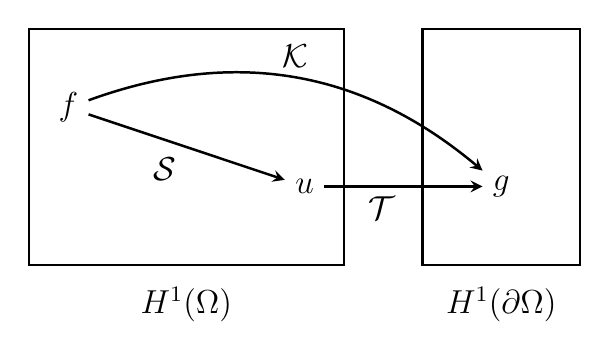
\begin{tikzpicture}[
        >=stealth,
        line width=0.9pt,
        every node/.style={font=\large}
    ]
    % Boxes
    \draw (0,0) rectangle (4,3);
    \draw (5,0) rectangle (7,3);
    
    % Space labels H^1
    \node at (2,-0.5) {$H^1(\Omega)$};
    \node at (6,-0.5) {$H^1(\partial\Omega)$};
    
    % f, u, and y points
    \node (f) at (0.5,2) {$f$};
    \node (u) at (3.5,1) {$u$};
    \node (g) at (6,1) {$g$};
    
    % Operator S
    \draw[->]
      (f) -- (u)
      node[midway, below left] {$\mathcal S$};
    
    % Operator T
    \draw[->]
      (u) -- (g)
      node[midway, below, xshift=-2.8mm] {$\mathcal T$};
    
    % Operator K
    \draw[->]
      (f) to[out=20, in=140]
      node[midway, above] {$\mathcal{K}$}
      (g);
    \end{tikzpicture}
    \caption{The forward operator $\mathcal K = \mathcal T \circ \mathcal S$ which maps $f$ to $g$.}
    \label{fig:forward_operator}
\end{figure}